\documentclass[conference]{IEEEtran}

% ============================================================================
% IEEE ICEIB Conference Paper Draft (Overleaf-ready, pdfLaTeX compatible)
% Project: GridReserve Agent (Group 4)
% Note: Verify romanized author names, affiliations, and emails before
% final submission to IEEE ICEIB. Replace [TBD] placeholders in Section IV
% after formal experiments E1--E4 are executed.
% ============================================================================

\usepackage[T1]{fontenc}
\usepackage[utf8]{inputenc}
\usepackage{cite}
\usepackage{amsmath,amssymb,amsfonts}
\usepackage{algorithm}
\usepackage{algpseudocode}
\usepackage{graphicx}
\usepackage{booktabs}
\usepackage{array}
\usepackage{tabularx}
\usepackage{microtype}
\usepackage[hyphens]{url}
\usepackage{xcolor}
\usepackage{tikz}
\usetikzlibrary{shapes.geometric, arrows.meta, positioning, fit, backgrounds}

% Mildly improve line breaking without changing IEEEtran page geometry.
\setlength{\emergencystretch}{1em}
\algrenewcommand\algorithmicindent{1.0em}

\def\BibTeX{{\rm B\kern-.05em{\sc i\kern-.025em b}\kern-.08em
    T\kern-.1667em\lower.7ex\hbox{E}\kern-.125emX}}

\begin{document}

\title{GridReserve Agent: A Tool-Constrained Domain AI Agent for Weather-Driven Load Forecasting and Outage Scenario Analysis in Taiwan's Power Grid}

% NOTE: Verify official romanized names, department affiliations, and emails.
\author{
\IEEEauthorblockN{Yu-Cen Lin, Hsuan-Yu Chen, and Chia-Shang Wang}
\IEEEauthorblockA{\textit{Department of Information / AIoT Course Project (Group 4)} \\
\textit{University / Institution [TBD]} \\
City, Taiwan \\
\{yucen.lin, hsuanyu.chen, chiashang.wang\}@example.edu.tw}
}

\maketitle

\begin{abstract}
Taiwan's power grid faces mounting operational pressure from semiconductor and artificial intelligence (AI) electricity growth alongside severe supply-side volatility. Taiwan Power Company (Taipower) projects the 2026 summer daytime peak load at $4{,}294 \times 10^4\text{ kW}$ ($42{,}940\text{ MW}$) and the night peak at $3{,}853 \times 10^4\text{ kW}$ ($38{,}530\text{ MW}$), both historic highs. Meanwhile, generator outages in September 2025--including the Hsinta New Unit 2 trial-operation explosion and Linkou Unit 2 trip--removed $210 \times 10^4\text{ kW}$ ($2{,}100\text{ MW}$, roughly $6\%$ of night peak) and drove operating reserve rates down toward $4\%$. Although Taipower and the Central Weather Administration (CWA) publish extensive operational and meteorological records, three critical gaps hinder public risk analysis: (1) operating reserve rate is a post-dispatch outcome nearly uncorrelated with temperature ($r \approx -0.07$), making direct time-series or weather-based prediction unreliable; (2) day-peak versus night-peak definitions and fast- versus slow-ramping reserve quality are absent from raw headline numbers; and (3) existing large language model (LLM) power-grid agents focus on synthetic power-flow simulators rather than public operational data, while unconstrained LLMs risk numerical hallucination. To address these gaps, we present \textbf{GridReserve Agent}, a tool-constrained Domain AI Agent grounded in Taiwan's public operational data. Our decoupled architecture delegates predictable peak load intervals ($10\%/50\%/90\%$ quantiles with conformal calibration) to weather- and calendar-driven machine learning models, while delegating unpredictable supply shocks and five-tier indicator lights to deterministic scenario simulation and domain rules. An LLM planner orchestrates task decomposition and natural-language explanation, subject to a mandatory verification gate that rejects ungrounded numbers or triggers safe refusal when queries exceed data coverage. We design an empirical evaluation protocol across $1{,}339$ merged daily records (2023-01-01 to 2026-08-31), a retrospective backtest of the September 2025 outages, and a $40$-question benchmark comparing pure LLMs, RAG-augmented LLMs, and our verification-gated agent. Preliminary exploratory analysis confirms strong weather-load correlation ($r \approx 0.75$), validates data-cleaning corrections for six erroneous official reserve entries, and establishes the feasibility of decoupled load forecasting and outage scenario reasoning while transparently reporting structural data limitations.
\end{abstract}

\begin{IEEEkeywords}
Domain AI agent, operating reserve margin, peak load forecasting, outage scenario analysis, numerical traceability, Taiwan power grid.
\end{IEEEkeywords}

\section{Introduction}
\label{sec:introduction}

In March 2026, Taiwan Power Company (Taipower) projected a record summer daytime peak load of $4{,}294 \times 10^4\text{ kW}$ ($42{,}940\text{ MW}$, up $4.89\%$ from $4{,}092 \times 10^4\text{ kW}$ in 2025) and a record night peak of $3{,}853 \times 10^4\text{ kW}$ ($38{,}530\text{ MW}$), driven primarily by rapid expansion in semiconductor manufacturing, servers, and cloud/AI workloads~\cite{ref7}. To sustain grid reliability, Taipower set operational reserve targets of $10\%$ for daytime peaks and at least $7\%$ for night peaks, alongside an unprecedented schedule of four large new generating units totaling over $500 \times 10^4\text{ kW}$ ($5{,}000\text{ MW}$) entering trial operation concurrently~\cite{ref7,ref8}. However, Ministry of Economic Affairs (MOEA) projections place 2025--2029 peak reserve margins between $11.3\%$ and $14.2\%$---below the $15\%$ planning benchmark---and unplanned generator faults in September 2025 caused actual reserve margins to plunge from a projected $14\%$ down to approximately $4\%$~\cite{ref9}.

Electric power systems require continuous instantaneous balancing of supply and demand. Taipower quantifies daily dispatchable supply adequacy using \textit{operating reserve capacity} $R = S - L$, where $S$ denotes net peak supply capability and $L$ denotes instantaneous peak load, and \textit{operating reserve rate} $r = (R / L) \times 100\%$~\cite{ref11}. Throughout this paper, we follow Taipower's standard operational unit of $10^4\text{ kW}$ ($10\text{ MW}$). Based on $R$ and $r$, Taipower issues a five-tier power supply status light: Green ($r \ge 10\%$), Yellow ($6\% < r < 10\%$), Orange ($r \le 6\%$), Red ($R \le 90 \times 10^4\text{ kW}$), and Black ($R \le 50 \times 10^4\text{ kW}$)~\cite{ref11}. Notably, since 2022 (ROC year 111), Taipower's historical annual reserve statistics have been reported using the nighttime peak basis~\cite{ref4}. Operational telemetry originates from Taipower's Energy Management System (EMS)~\cite{ref30} and Central Weather Administration (CWA) meteorological stations~\cite{ref6}.

Despite the public availability of these sensing and operational streams, researchers, policy analysts, and the public still lack a transparent, verifiable tool to answer practical contingency questions such as: \textit{``What is the expected peak load tomorrow, what happens to the operating reserve and indicator light if a major thermal unit trips, and which units contributed to a past low-reserve event?''} Four fundamental limitations prevent existing approaches from solving this problem reliably:

\begin{enumerate}
    \item \textbf{Direct reserve rate forecasting is unreliable.} Exploratory analysis across $1{,}339$ historical days shows that peak load correlates strongly with three-station mean daily maximum temperature ($r \approx 0.75$), whereas operating reserve rate correlates at only $r \approx -0.07$ with temperature. Because net peak supply capability $S$ is co-scheduled with anticipated demand ($r_{S,L} \approx 0.92$), directly predicting $r$ from weather yields worse accuracy than naive historical averages.
    \item \textbf{Headline reserve numbers mask operational quality.} During Taiwan's May 13 and May 17 blackout incidents, nominal operating reserve stood near $10\%$, yet fast-start capacity accounted for roughly $2\%$, while coal restarts, depleted pumped-storage hydro, and sunsetting solar PV curtailed actual responsive margin~\cite{ref14}.
    \item \textbf{Official forecasts diverge from outage realities.} During the September 2025 Hsinta and Linkou unit failures, sudden generation losses rapidly eroded projected adequacy down to near-emergency conditions~\cite{ref9,ref10,ref12,ref13}.
    \item \textbf{Existing LLM grid agents address different abstractions.} Recent LLM-based power system agents such as GridMind~\cite{ref20}, X-GridAgent~\cite{ref21}, and Grid-Agent~\cite{ref22} coordinate power-flow or optimal power flow (OPF) solvers over IEEE synthetic bus benchmarks. Literature surveys highlight limited operational datasets, insufficient explainability, a disconnect between single-metric forecasting and decision contexts, and numerical hallucination risks in safety-critical domains~\cite{ref23,ref24}.
\end{enumerate}

To bridge these gaps, we propose \textbf{GridReserve Agent}, a tool-constrained Domain AI Agent tailored to Taiwan's public power and weather data. Our work makes five core contributions:
\begin{itemize}
    \item \textbf{Decoupled Forecasting and Contingency Architecture:} We assign weather-sensitive peak load interval forecasting to machine learning while delegating volatile supply shocks and regulatory indicator logic to deterministic scenario simulation, avoiding naive reserve-rate regression.
    \item \textbf{Reusable Taiwan Grid Domain Knowledge Base:} We codify Taipower's dual-logic indicator rules (separating absolute thresholds for Red/Black lights from ratio thresholds for Green/Yellow/Orange lights), an enriched $175$-unit equipment inventory with fast/slow ramp annotations, day-versus-night peak caveats, and an $N\text{-}1$ single-largest-unit adequacy ratio ($R / C_{\max}$).
    \item \textbf{Public Data Quality Auditing and Cleaning Pipeline:} We identify and systematically correct six anomalous reserve-rate entries in Taipower's main supply-demand dataset (e.g., $202.0\%$ corrected to $20.2\%$), handle trace rainfall encodings ($-9.8 \rightarrow 0$), standardize units, and reconstruct 2023--2024 peak loads with $0.014\%$ mean relative error.
    \item \textbf{Verification-Gated Agent Control Flow:} Our LLM planner handles intent parsing, task decomposition, and explanation, but is prohibited from fabricating numerical values; every figure must pass a post-hoc traceability check against tool outputs or trigger bounded regeneration and safe refusal/failure.
    \item \textbf{Reproducible Evaluation Protocol and Open-Source Blueprint:} We establish a multi-faceted benchmark (Experiments E1--E4) spanning rolling load forecasting, September 2025 outage backtesting, a $40$-question traceability/hallucination suite, and boundary unit testing, alongside full design specifications.
\end{itemize}

The remainder of this paper is organized as follows. Section~\ref{sec:related_work} reviews AI power-grid agents, load forecasting methods, and Taiwan domain knowledge, culminating in a structured research gap analysis. Section~\ref{sec:proposed_design} details the domain mental models, eight-module architecture, mathematical formulation, and core algorithms. Section~\ref{sec:experiment} presents the datasets, preliminary exploratory feasibility observations, and the E1--E4 evaluation design. Section~\ref{sec:conclusion} concludes with system limitations and future research directions.

\section{Related Work}
\label{sec:related_work}

This section surveys two complementary pillars: AI/LLM techniques for power systems and domain-specific operational knowledge of Taiwan's grid.

\subsection{AI Technologies for Power Systems}
\label{sec:related_ai}

\textbf{LLM Power-Grid Agents.} Recent multi-agent systems integrate semantic reasoning with deterministic numerical engines. GridMind combines LLM agents with power-system solvers to execute natural-language optimal power flow (OPF) and $N\text{-}1$ contingency analyses across IEEE 14- to 300-bus test cases~\cite{ref20}. X-GridAgent introduces a hierarchical planning, coordination, and execution architecture leveraging Model Context Protocol (MCP) tools and knowledge bases on a $2{,}000$-bus Texas grid~\cite{ref21}. Grid-Agent pairs a planning agent with a validation agent to detect and remediate voltage and thermal violations on IEEE 30/69 and CIGRE MV networks~\cite{ref22}. A 2026 comparative study on agentic smart grids further emphasizes verification gates and safe failure mechanisms~\cite{ref25}. Collectively, these architectures establish the principle that LLMs should orchestrate tools rather than perform numerical computation directly.

\textbf{Reliability, Decision Alignment, and Hallucination.} Comprehensive surveys of LLMs in power systems identify limited public domain data, operational reliability, and interpretability as primary deployment barriers~\cite{ref23}. A 2026 survey on LLM-agent renewable forecasting notes that conventional predictors optimize isolated point-error metrics without linking outputs to reserve procurement or dispatch decisions, and warns that while LLMs excel at communication, unverified numerical outputs pose severe hallucination risks~\cite{ref24}.

\textbf{Load, Net-Load, and Probabilistic Forecasting.} In the Taiwanese context, researchers at National Taiwan University evaluated hourly Taipower load and renewable data using hybrid SARIMAX, NNARX, and functional data analysis (FPCA) models~\cite{ref26}, while a 2023 study demonstrated that a temperature-aware hybrid convolutional neural network (CNN) outperformed MLP, RNN, VARMA, and SVM on week-ahead Taiwan daily peak load forecasting~\cite{ref27}. For risk-aware operations, quantile regression forests and conformal prediction provide calibrated prediction intervals directly usable for reserve adequacy decisions~\cite{ref24}.

\subsection{Taiwan Grid Domain Know-How}
\label{sec:related_domain}

\textbf{Reserve Definitions, Quality, and Peak Shifts.} Official Taipower guidelines define the five-tier reserve indicator rules~\cite{ref11}, while historical statistics reflect the transition to nighttime peak reserve reporting since 2022~\cite{ref4}. Domain analyses of the May 13 and May 17 blackouts illustrate why reserve quantity diverges from responsive quality when thermal units require hours to ramp and solar generation declines rapidly at dusk~\cite{ref14}, and reporting on Taiwan's 2025 supply crunch warns that evening reserve margins could compress sharply under tight summer conditions~\cite{ref15}.

\textbf{Duck Curve, Unit Commitment, and Grid Incidents.} Optimization studies on Taiwan's energy transition highlight how high solar penetration reshapes daily net load into a duck curve, elevating pumped-storage hydro as critical daytime storage~\cite{ref28}, while probabilistic duck-curve modeling captures net-load ramping uncertainty~\cite{ref29}. Operational risks materialized in September 2025 when a gas-leak fire/explosion during trial testing at Hsinta New Unit 2, combined with Linkou Unit 2 and Unit 1 failures, cut $210$ to $290 \times 10^4\text{ kW}$ of supply~\cite{ref10,ref12,ref13}. Taipower's expansion roadmap relies on Hsinta's three new gas units ($390 \times 10^4\text{ kW}$ total)~\cite{ref18} and four large new units (Hsinta New Units 2--3 and Taichung New Units 1--2, each Taichung unit rated at $130 \times 10^4\text{ kW}$) entering commercial operation in 2026~\cite{ref19,ref31}. Our system integrates six public datasets spanning Taipower supply-demand records, forecasts, unit inventories, 10-minute unit logs, and CWA weather observations~\cite{ref1,ref2,ref3,ref4,ref5,ref6,ref30}.

\begin{table*}[t]
\centering
\caption{Comparative Summary of Related Studies Across AI Power-Grid Agents, Load Forecasting, and Taiwan Domain Analysis}
\label{tab:related_work}
\renewcommand{\arraystretch}{1.15}
\begin{tabularx}{\textwidth}{@{}p{1.55cm}cp{2.1cm}>{\raggedright\arraybackslash}X>{\raggedright\arraybackslash}X p{1.9cm}>{\raggedright\arraybackslash}X>{\raggedright\arraybackslash}X@{}}
\toprule
\textbf{Ref.} & \textbf{Year} & \textbf{Problem} & \textbf{AI Method} & \textbf{Domain Focus} & \textbf{Dataset} & \textbf{Key Findings} & \textbf{Limitation} \\
\midrule
\cite{ref20} GridMind & 2025 & Natural-language grid analysis & LLM multi-agent + deterministic solver & Optimal power flow, $N\text{-}1$ & IEEE 14--300 buses & Integrates LLM with solvers & Simulation-centric; no Taiwan public data \\
\cite{ref21} X-GridAgent & 2025 & Lowering power analysis barrier & Hierarchical planner/executor, MCP, KB & Power flow analysis & Texas 2k-bus & Natural-language execution & Assumes steady-state grid \\
\cite{ref22} Grid-Agent & 2025 & Automated violation remediation & Planner + validator multi-agent & Voltage \& overload limits & IEEE 30/69, CIGRE MV & Combines semantic \& numerical precision & Power-flow repair, not reserve adequacy \\
\cite{ref23} Survey & 2025 & LLMs in power systems & Literature survey & Grid operations & N/A & Identifies data, trust, XAI gaps & Conceptual survey; no system \\
\cite{ref24} Survey & 2026 & Forecast-decision gap \& hallucination & Quantile RF, conformal, LLM agent & Reserve procurement & N/A & Proposes hybrid agent architecture & Survey only; no Taiwan deployment \\
\cite{ref26} Taiwan Netload & 2025 & Load and net-load forecasting & SARIMAX, NNARX, FPCA hybrid & Renewables \& weather & Taipower hourly load/RE & Benchmarks statistical vs. ML & Forecasts load only; no outage scenarios \\
\cite{ref27} Peak Load & 2023 & Week-ahead peak forecasting & Hybrid CNN & Temperature effects & Taiwan daily peak \& weather & Outperforms MLP, RNN, VARMA, SVM & Point forecast only; no decision link \\
\cite{ref28} Taiwan UC & 2020 & High-RE unit commitment & Optimization (AMPL/CPLEX) & Duck curve, pumped hydro & Taiwan scenario model & Pumped hydro mitigates duck curve & Planning layer, not daily risk tool \\
\cite{ref29} Prob. Duck & 2019 & PV ramping uncertainty & Probabilistic modeling & Duck curve, ramping & Qinghai, China & Quantifies net-load uncertainty & Non-Taiwan power system \\
\cite{ref14} 513/517 Analysis & 2022 & Evaluating reserve overestimation & Investigative analysis & Fast/slow reserve, solar PV & Media \& EMS reports & Highlights gap in rapid dispatchability & Qualitative reporting; needs verification \\
\midrule
\textbf{Ours} & \textbf{2026} & \textbf{Taiwan reserve risk analysis} & \textbf{ML quantiles + LLM planner + verify gate} & \textbf{Lights, $N\text{-}1$, unit KB, day/night} & \textbf{1,339-day Taipower + CWA} & \textbf{Decoupled forecast, outage sim, zero-hallucination gate} & \textbf{No direct night reserve in public CSVs} \\
\bottomrule
\end{tabularx}
\end{table*}

\subsection{Research Gap}
\label{sec:research_gap}

As summarized in Table~\ref{tab:related_work}, existing LLM grid agents~\cite{ref20,ref21,ref22} operate on synthetic steady-state bus models rather than national public dispatch datasets, whereas Taiwan forecasting and scheduling studies~\cite{ref26,ref27,ref28} lack interactive contingency reasoning, indicator-light semantics, and hallucination safeguards. Consequently, a clear research gap remains for a domain-grounded, tool-constrained AI agent capable of probabilistic peak load forecasting, generator outage scenario simulation, historical low-reserve attribution, and strictly traceable explanation over Taiwan's public operational data.

\section{Proposed Design}
\label{sec:proposed_design}

\subsection{Domain Mental Models and Design Principles}
\label{sec:mental_models}

To prevent superficial metric optimization, GridReserve Agent embeds five domain mental models (M1--M5) derived from Taiwan grid operations and three structural policy debates (whether a $10\%$ vs. $6\%$ reserve threshold suffices~\cite{ref11,ref16,ref17}, whether nominal reserves overstate fast-dispatchable supply~\cite{ref14}, and whether official forecasts underestimate outage/delay risks~\cite{ref7,ref8,ref9,ref10}):
\begin{itemize}
    \item \textbf{M1 (Reserve as Insurance):} Operating reserve trades reliability against fuel cost and emissions (e.g., Hsinta coal units restricted by environmental permits to operate only below $8\%$ reserve~\cite{ref18}). Thus, outputs frame risk trade-offs rather than advocating arbitrarily high reserves.
    \item \textbf{M2 (Quality Over Quantity):} Fast-ramping units differ fundamentally from slow thermal plants~\cite{ref14}; our knowledge base explicitly annotates fuel type and fast/slow response classes.
    \item \textbf{M3 ($N\text{-}1$ Single-Unit Contingency):} Adequacy must survive the sudden trip of the largest online unit ($C_{\max} = 130 \times 10^4\text{ kW}$), motivated by the September 2025 ($210 \times 10^4\text{ kW}$) and August 15 Tatan ($\sim 8\%$) outages~\cite{ref10,ref17}.
    \item \textbf{M4 (Day vs. Night Peak Semantics):} Daytime peaks benefit from solar PV, whereas night peaks do not~\cite{ref4,ref7,ref8}. Every output explicitly tags peak type and data-coverage boundaries.
    \item \textbf{M5 (Uncertainty-Linked Decisions):} Point forecasts are insufficient for dispatch risk~\cite{ref24,ref29}; our load engine outputs $10\%/50\%/90\%$ conformal intervals.
\end{itemize}

\subsection{Eight-Module System Architecture}
\label{sec:architecture}

Fig.~\ref{fig:architecture} illustrates the eight-module architecture of GridReserve Agent, separating natural-language orchestration from deterministic computation and validation.

\begin{figure*}[t]
\centering
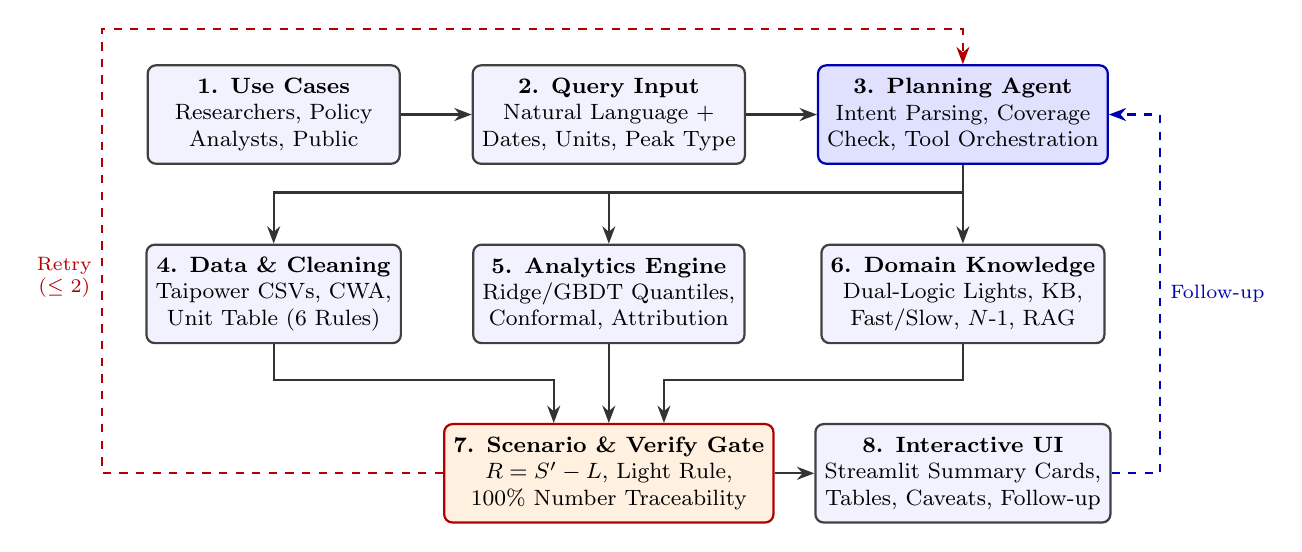
\begin{tikzpicture}[
    node distance=0.8cm and 0.9cm,
    box/.style={rectangle, rounded corners=3pt, draw=black!75, fill=blue!5, thick, minimum width=3.2cm, minimum height=1.25cm, align=center, font=\footnotesize},
    core/.style={rectangle, rounded corners=3pt, draw=blue!70!black, fill=blue!12, thick, minimum width=3.4cm, minimum height=1.25cm, align=center, font=\footnotesize},
    gate/.style={rectangle, rounded corners=3pt, draw=red!70!black, fill=orange!12, thick, minimum width=3.4cm, minimum height=1.25cm, align=center, font=\footnotesize},
    arrow/.style={-{Stealth[length=2.2mm]}, thick, draw=black!80}
]

% Top Row: 1 -> 2 -> 3
\node[box] (m1) {\textbf{1. Use Cases}\\Researchers, Policy\\Analysts, Public};
\node[box, right=of m1] (m2) {\textbf{2. Query Input}\\Natural Language +\\Dates, Units, Peak Type};
\node[core, right=of m2] (m3) {\textbf{3. Planning Agent}\\Intent Parsing, Coverage\\Check, Tool Orchestration};

% Middle Row: 4, 5, 6
\node[box, below=1.0cm of m1] (m4) {\textbf{4. Data \& Cleaning}\\Taipower CSVs, CWA,\\Unit Table (6 Rules)};
\node[box, below=1.0cm of m2] (m5) {\textbf{5. Analytics Engine}\\Ridge/GBDT Quantiles,\\Conformal, Attribution};
\node[box, below=1.0cm of m3] (m6) {\textbf{6. Domain Knowledge}\\Dual-Logic Lights, KB,\\Fast/Slow, $N\text{-}1$, RAG};

% Bottom Row: 7 -> 8
\node[gate, below=1.0cm of m5] (m7) {\textbf{7. Scenario \& Verify Gate}\\$R=S'-L$, Light Rule,\\100\% Number Traceability};
\node[box, below=1.0cm of m6] (m8) {\textbf{8. Interactive UI}\\Streamlit Summary Cards,\\Tables, Caveats, Follow-up};

% Outer corridors for clean non-crossing feedback loops
\coordinate (leftcorridor) at ([xshift=-0.55cm]m4.west);
\coordinate (rightcorridor) at ([xshift=0.65cm]m3.east);

% Arrows
\draw[arrow] (m1) -- (m2);
\draw[arrow] (m2) -- (m3);
\draw[arrow] (m3.south) -- ++(0,-0.35) -| (m4.north);
\draw[arrow] (m3.south) -- ++(0,-0.35) -| (m5.north);
\draw[arrow] (m3.south) -- (m6.north);

\draw[arrow] (m4.south) -- ++(0,-0.45) -| ([xshift=-0.7cm]m7.north);
\draw[arrow] (m5.south) -- (m7.north);
\draw[arrow] (m6.south) -- ++(0,-0.45) -| ([xshift=0.7cm]m7.north);

\draw[arrow] (m7) -- (m8);
\draw[arrow, dashed, blue!70!black] (m8.east) -- (rightcorridor |- m8.east) -- (rightcorridor) node[midway, right, font=\scriptsize] {Follow-up} -- (m3.east);
\draw[arrow, dashed, red!70!black] (m7.west) -- (leftcorridor |- m7.west) |- ([yshift=0.45cm]m3.north) node[pos=0.22, left, align=center, font=\scriptsize] {Retry\\($\le 2$)} -- (m3.north);

\end{tikzpicture}
\caption{Eight-module architecture of GridReserve Agent. The LLM planner (Module 3) invokes deterministic data, analytics, and knowledge tools (Modules 4--6), while the verification gate (Module 7) enforces numerical traceability prior to output (Module 8).}
\label{fig:architecture}
\end{figure*}

\begin{enumerate}
    \item \textbf{Use Cases (Module 1):} Supports researchers, policy analysts, and the general public on forecast, outage, diagnosis, and conceptual queries.
    \item \textbf{Query Input (Module 2):} Accepts natural-language questions paired with optional structured parameters (target date, plant/unit name, outage scenario, and peak type).
    \item \textbf{Planning and Reasoning Agent (Module 3):} An LLM classifier maps queries into four intents---\texttt{FORECAST}, \texttt{WHATIF}, \texttt{DIAGNOSE}, or \texttt{EXPLAIN}---and decomposes subtasks. If entities fall outside verified data coverage (e.g., direct night-peak reserve queries, out-of-range dates, or uncovered private independent power producers [IPPs]), the agent triggers immediate safe refusal with an explicit explanation.
    \item \textbf{Data Acquisition and Cleaning (Module 4):} Ingests six raw CSV files (three Taipower files and three CWA station files) under six deterministic cleaning rules: (a) recompute operating reserve rate $r = (R / L) \times 100\%$ to eliminate six magnitude errors (such as $202.0\%$ corrected to $20.2\%$, spanning four cross-verified 2025 dates and two 2026 dates); (b) map trace precipitation code $-9.8$ to $0$ and discard unused meteorological fields (retaining $\sim 10$ features from $279$ raw columns per station); (c) drop six all-zero decommissioned/inactive unit columns (Chinshan, Kuosheng, Maanshan \#1, Mailiao \#2, etc.); (d) standardize capacities from $\text{kW}$ to $10^4\text{ kW}$; (e) parse \texttt{YYYYMMDD} integers and merge the 2023--2025 three-year file with the 2025--2026 main file using $365$ overlapping 2025 days for validation; and (f) reverse-compute 2023--2024 peak load $L = R / (r/100)$ and net supply $S = L + R$.
    \item \textbf{Analytics Engine (Module 5):} Trains Ridge Regression and Gradient Boosting models using calendar features (day-of-week, month, holiday indicators, trend) and three-station meteorological observations (maximum/mean temperature, humidity, precipitation, sunshine duration) to produce $10\%$, $50\%$, and $90\%$ load quantiles calibrated via conformal prediction. To prevent data leakage, same-day generator, solar, and wind outputs are strictly excluded from forecasting features and reserved solely for post-hoc low-reserve attribution ($r < 10\%$), which compares an event day against the trailing $7$-week same-weekday average and labels the caveat that generation output delta does not equal available capacity.
    \item \textbf{Domain Knowledge Base (Module 6):} Encodes five-tier indicator rules as declarative configuration, maintains the $175$-unit equipment catalog ($\sim 2{,}963 \times 10^4\text{ kW}$) supplemented with Hsinta New Units ($3$ units, $390 \times 10^4\text{ kW}$~\cite{ref18}) and Taichung New Units 1 and 2 ($130 \times 10^4\text{ kW}$ each~\cite{ref31}), computes the $N\text{-}1$ ratio against $C_{\max} = 130 \times 10^4\text{ kW}$, and serves a curated retrieval-augmented generation (RAG) corpus of public policy reports.
    \item \textbf{Scenario Simulation and Verification Gate (Module 7):} Computes outage-adjusted reserve capacity, reserve rate, and light status purely via deterministic functions, then verifies that every numeric token in the LLM-authored narrative matches a tool output identifier, unit, and date. Failed checks trigger up to two regeneration retries before falling back to a safe failure message.
    \item \textbf{Output and Interaction (Module 8):} Presents grounded summary cards, tables, charts, uncertainty bounds, citations, and explicit data limitations in a Streamlit interface supporting follow-up questions.
\end{enumerate}

\subsection{Mathematical Formulation and Dual-Logic Indicator Rules}
\label{sec:formulation}

For a target date $d$ and a hypothetical outage unit set $\mathcal{U}_{\text{out}}$, let $S_{\text{ref}}(d)$ denote the reference net peak supply capability (obtained from Taipower's two-month forecast~\cite{ref2} when available, or the recent same-weekday median), and let $\hat{L}_{q}(d)$ denote the predicted peak load at quantile $q \in \{0.10, 0.50, 0.90\}$. The outage-adjusted supply $S'(d)$, operating reserve capacity $R(d)$, operating reserve rate $r(d)$, and $N\text{-}1$ adequacy ratio $\eta_{N-1}(d)$ are computed as:
\begin{equation}
S'(d) = S_{\text{ref}}(d) - \sum_{u \in \mathcal{U}_{\text{out}}} C_u,
\label{eq:supply}
\end{equation}
\begin{equation}
R(d) = S'(d) - \hat{L}(d), \qquad r(d) = \frac{R(d)}{\hat{L}(d)} \times 100\%,
\label{eq:reserve}
\end{equation}
\begin{equation}
\eta_{N-1}(d) = \frac{R(d)}{C_{\max}}, \quad C_{\max} = 130 \times 10^4\text{ kW},
\label{eq:n1}
\end{equation}
where $C_u$ is the installed capacity of unit $u$ in $10^4\text{ kW}$. Evaluating~\eqref{eq:supply}--\eqref{eq:reserve} across $\hat{L}_{0.10}$, $\hat{L}_{0.50}$, and $\hat{L}_{0.90}$ yields probabilistic bounds on reserve erosion and light transitions.

Crucially, Taipower's five-tier indicator logic exhibits precedence between absolute capacity thresholds and percentage thresholds: absolute capacity checks ($R \le 50$ for Black, $R \le 90$ for Red) strictly precede ratio checks ($r \le 6\%$ for Orange, $r < 10\%$ for Yellow, otherwise Green). For example, if $R = 85 \times 10^4\text{ kW}$ and $r \approx 2.4\%$, the system must emit \texttt{RED} rather than \texttt{ORANGE}.

\subsection{Agent Control Flow and Algorithms}
\label{sec:algorithms}

The operational logic incorporates three decision points (data coverage validation, intent routing, and traceability verification) and two feedback loops (up to two regeneration attempts and multi-turn user follow-ups). Algorithms~\ref{alg:agent} and~\ref{alg:light} formalize the end-to-end execution and dual-logic indicator classification.

\begin{algorithm}[t]
\footnotesize
\caption{GridReserve Agent Execution Pipeline}
\label{alg:agent}
\begin{algorithmic}[1]
\Require User query $Q$
\Ensure Grounded response $R_{\text{out}}$ with evidence,
\Statex \hspace{\algorithmicindent} uncertainty, and limitations
\State Parse intent $I$ and entities $E$ from $Q$
\Statex \hspace{\algorithmicindent} $I \in \{\text{FORECAST}, \text{WHATIF}, \text{DIAGNOSE}, \text{EXPLAIN}\}$
\If{$E$ is outside verified data coverage}
    \Statex \hspace{\algorithmicindent} (dates, night peak, uncovered IPPs)
    \State \Return $\text{SafeRefusal}(\text{reason})$
\EndIf
\State $P \gets \text{Decompose}(I, E)$
\State $D \gets \text{LoadAndClean}(\text{sources})$ \Comment{6 cleaning rules, $10^4\text{ kW}$}
\For{each subtask $t \in P$}
    \If{$t$ is LoadForecast}
        \State $(\hat{L}, \text{band}) \gets \text{ForecastLoad}($
        \Statex \hspace{\algorithmicindent} $E.\text{dates}, \text{weather}, \text{calendar})$
    \ElsIf{$t$ is Scenario}
        \State $S' \gets \text{RefSupply}(E.\text{dates}) - \sum_{u \in E.\text{outage}} C_u$
    \ElsIf{$t$ is Diagnose}
        \State $\text{top\_k} \gets \text{Attribute}(E.\text{date},$
        \Statex \hspace{\algorithmicindent} $\text{same weekday}, \text{7 weeks})$
    \EndIf
\EndFor
\State $R_{\text{cap}} \gets S' - \hat{L}$
\State $r \gets (R_{\text{cap}} / \hat{L}) \times 100$
\State $\text{light} \gets \text{ClassifyLight}(R_{\text{cap}}, r)$
\Comment{Algorithm~\ref{alg:light}}
\State $\eta_{N-1} \gets R_{\text{cap}} / \text{MaxUnitCapacity}(\text{KB})$
\State $\text{notes} \gets \text{Retrieve}(\text{KB}, I, \text{light})$
\Comment{Quality, day/night, caveats}
\For{$\text{attempt} = 1$ \textbf{to} $3$} \Comment{Max 2 retries}
    \State $R_{\text{out}} \gets \text{Compose}(\text{results}, \text{notes}, \text{citations})$
    \If{$\text{Verify}(R_{\text{out}}, \text{tool\_outputs})$}
        \State \textbf{break}
    \EndIf
\EndFor
\If{not verified}
    \State \Return $\text{SafeFailure}()$
\EndIf
\State \Return $R_{\text{out}}$ with evidence, uncertainty,
\Statex \hspace{\algorithmicindent} and limitations
\end{algorithmic}
\end{algorithm}

\begin{algorithm}[t]
\footnotesize
\caption{ClassifyLight: Dual-Logic Power Supply Status}
\label{alg:light}
\begin{algorithmic}[1]
\Require Reserve capacity $R_{\text{cap}}$ ($10^4\text{ kW}$),
\Statex \hspace{\algorithmicindent} reserve rate $r$ ($\%$)
\Ensure Supply indicator tier $\text{light}$ belongs to:
\Statex \hspace{\algorithmicindent} $\{\text{BLACK}, \text{RED}, \text{ORANGE},$
\Statex \hspace{\algorithmicindent} $\text{YELLOW}, \text{GREEN}\}$
\If{$R_{\text{cap}} \le 50$}
    \State \Return \texttt{BLACK}
\EndIf
\If{$R_{\text{cap}} \le 90$}
    \State \Return \texttt{RED}
\EndIf
\If{$r \le 6$}
    \State \Return \texttt{ORANGE}
\EndIf
\If{$r < 10$}
    \State \Return \texttt{YELLOW}
\EndIf
\State \Return \texttt{GREEN}
\end{algorithmic}
\end{algorithm}

\section{Experiment and Evaluation}
\label{sec:experiment}

\subsection{Datasets and Cleaning Verification}
\label{sec:datasets}

Table~\ref{tab:datasets} summarizes the five public operational, meteorological, and equipment datasets integrated into GridReserve Agent. After merging the 3-year historical reserve file~\cite{ref3} ($1{,}096$ days, 2023-01-01 to 2025-12-31) with the main supply-demand file~\cite{ref1} ($608$ days, 2025-01-01 to 2026-08-31), the unified corpus covers $1{,}339$ consecutive days, paired with daily CWA observations~\cite{ref6} from Taipei (`466920`), Taichung (`467490`), and Kaohsiung (`467441`).

\begin{table}[t]
\centering
\caption{Public Datasets Integrated into GridReserve Agent}
\label{tab:datasets}
\footnotesize
\renewcommand{\arraystretch}{1.12}
\setlength{\tabcolsep}{2pt}
\begin{tabularx}{\columnwidth}{@{}p{1.25cm}r p{1.45cm}>{\raggedright\arraybackslash}X@{}}
\toprule
\textbf{Dataset} & \textbf{Records} & \textbf{Period} & \textbf{Role and Data Issues} \\
\midrule
3-Year Daily Reserve \cite{ref3} & 1,096 & 2023-01--2025-12 & Primary reserve history; clean and continuous \\
Past Supply \& Demand \cite{ref1} & 608 & 2025-01--2026-08 & Unit, PV, and wind output; 6 reserve-rate errors \\
2-Month Forecast \cite{ref2} & 6 & 2026-11--2026-12 & Display only (10-day intervals); no backtest \\
CWA Daily Weather \cite{ref6} & 1,339 ($\times 3$) & 2023-01--2026-08 & Taipei, Taichung, and Kaohsiung; trace rain $-9.8$ \\
Unit Inventory \cite{ref5} & 175 units & Static (to 2023-06) & Unit KB; lacks new gas units, IPPs, and 52 six-digit CODs \\
\bottomrule
\end{tabularx}
\end{table}

\subsection{Preliminary Exploratory Feasibility Analysis}
\label{sec:preliminary_eda}

Before executing formal evaluations, we conducted exploratory data analysis (EDA) across the $1{,}339$-day dataset strictly to validate data integrity and modeling assumptions (these observations are preliminary diagnostics rather than formal experiment results):

\begin{itemize}
    \item \textbf{Reverse-Computation Accuracy:} Over the $365$ overlapping days in 2025 between~\cite{ref3} and~\cite{ref1}, reverse-computing peak load via $L = R / (r/100)$ achieved a mean relative error of approximately $0.014\%$, validating reconstruction of 2023--2024 demand.
    \item \textbf{Anomaly Detection and Indicator Distribution:} Recomputing $r$ corrected six $10\times$-scaled anomalies in~\cite{ref1} (2025-03-29, 2025-04-27, 2025-10-20, 2025-10-25 cross-checked with~\cite{ref3}; 2026-04-05, 2026-04-17 corrected directly). Across $1{,}096$ days in~\cite{ref3}, light counts are $1{,}046$ Green, $50$ Yellow, and $0$ Orange; across $608$ cleaned days in~\cite{ref1}, counts are $573$ Green, $35$ Yellow, and $0$ Orange, with a minimum reserve rate of $6.08\%$ on 2025-09-23.
    \item \textbf{Correlation Structure and Predictability:} Peak load exhibits strong temperature coupling ($r \approx 0.75$), and supply tracks load closely ($r \approx 0.92$), whereas operating reserve rate exhibits negligible temperature correlation ($r \approx -0.07$). Simple reserve-rate baselines (previous day, previous week, monthly mean) incur $\text{MAE} \approx 5.8\text{--}6.2$ percentage points ($\sigma \approx 6.6$) with no improvement from adding temperature. Conversely, exploratory linear load models on test dates from 2025-09-01 onward reduced MAE to $\sim 100\text{--}150 \times 10^4\text{ kW}$ compared to a mean-guessing baseline of $\sim 367 \times 10^4\text{ kW}$.
    \item \textbf{September 2025 Incident Trace:} Operational logs confirm Linkou Unit 2 output dropped to $0$ from September 15, 2025 onward, coinciding with tight reserve rates of $6.11\%$ on September 18 and $6.08\%$ on September 23.
\end{itemize}

\subsection{Experimental Protocol (E1--E4)}
\label{sec:protocol}

To rigorously evaluate forecasting precision, contingency fidelity, agent trustworthiness, and rule compliance, we define four experiments (E1--E4) summarized in Table~\ref{tab:experiments}.

\begin{table*}[t]
\centering
\caption{Experimental Evaluation Protocol (E1--E4), Baselines, Metrics, and Current Completion Status}
\label{tab:experiments}
\renewcommand{\arraystretch}{1.15}
\begin{tabularx}{\textwidth}{@{}p{1.75cm}>{\raggedright\arraybackslash}X>{\raggedright\arraybackslash}X>{\raggedright\arraybackslash}Xp{1.75cm}@{}}
\toprule
\textbf{Exp.} & \textbf{Scope and Setup} & \textbf{Baselines} & \textbf{Evaluation Metrics} & \textbf{Status} \\
\midrule
\textbf{E1:} Load Forecasting & Train 2023-01-01 to 2025-08-31; rolling retrain test 2025-09-01 to 2026-08-31; plus weather-noise sensitivity & Monthly mean, prior-week same day, calendar-only (no weather) & MAE, MAPE, pinball loss, $80\%$ prediction interval coverage & Planned \texttt{[TBD]} \\
\textbf{E2:} Outage Backtest & September 2025 Hsinta \& Linkou outages; predict post-outage reserve from pre-incident state vs. actuals (Sep 9--23) & Unadjusted reference supply capability (no outage deduction) & Reserve drop error ($10^4\text{ kW}$), indicator light agreement & Planned \texttt{[TBD]} \\
\textbf{E3:} Agent QA & $40$ questions ($10$ forecast, $10$ scenario, $8$ diagnosis, $6$ explain, $6$ out-of-scope traps); programmatic ground truth & Pure LLM, LLM + RAG, Agent without verification gate (ablation) & Numeric accuracy ($1\%$ tol.), traceability, refusal accuracy, hallucination rate & Planned \texttt{[TBD]} \\
\textbf{E4:} Rule Tests & Exhaustive unit tests across indicator thresholds ($50, 90 \times 10^4\text{ kW}$; $6\%, 10\%$) and priority order & Deterministic test suite & Assertion pass rate ($\%$) & Planned \texttt{[TBD]} \\
\bottomrule
\end{tabularx}
\end{table*}

In E1, because CWA daily observations act as an oracle upper bound for weather forecasts, Gaussian forecast-error perturbations will be injected to assess sensitivity. Taipower's two-month forecast~\cite{ref2} ($6$ snapshots) is excluded as a backtest baseline and used only for November--December 2026 demonstration.

\subsection{Expected Outcomes and Formal Result Placeholders}
\label{sec:expected_outcomes}

Formal execution of E1--E4 is pending completion of the implementation pipeline. Accordingly, we report explicit placeholders rather than unverified figures:
\begin{itemize}
    \item \textbf{E1 Result \texttt{[TBD]}:} Weather-augmented Ridge/Gradient Boosting models are expected to substantially reduce MAE/MAPE relative to no-weather and calendar baselines while achieving calibrated $\approx 80\%$ conformal coverage; direct reserve-rate regression is expected to remain non-predictive and will be reported candidly.
    \item \textbf{E2 Result \texttt{[TBD]}:} Scenario deduction is expected to reproduce the direction and magnitude of reserve drop and Green-to-Yellow transitions during September 9--23, 2025.
    \item \textbf{E3 Result \texttt{[TBD]}:} The verification-gated agent is expected to approach $100\%$ numerical traceability and near-zero hallucination compared with pure LLM and unverified RAG baselines, alongside high refusal precision on the six out-of-scope traps.
    \item \textbf{E4 Result \texttt{[TBD]}:} Exhaustive boundary tests for \texttt{ClassifyLight} are expected to achieve $100\%$ pass rate.
\end{itemize}

\section{Conclusion and Future Work}
\label{sec:conclusion}

This paper presented the design and evaluation framework of \textbf{GridReserve Agent}, a tool-constrained Domain AI Agent for Taiwan's electric power reserve risk analysis. By decoupling weather-driven probabilistic peak load forecasting from deterministic outage scenario simulation, codifying Taiwan's dual-logic indicator rules and $N\text{-}1$ unit adequacy metrics, repairing six official dataset anomalies, and enforcing a strict post-generation verification gate, the architecture directly mitigates LLM numerical hallucination while addressing the non-stationarity of human-dispatched reserve margins.

Six practical limitations bound the current scope: (1) operating reserve rate is fundamentally a dispatch decision and cannot be reliably forecast solely from weather; (2) public daily datasets lack direct nighttime peak reserve values, requiring explicit peak-type labeling; (3) Taipower's static unit inventory ends at June 27, 2023 and omits IPPs, wind, and solar plants, requiring manual supplementation of new gas units; (4) historical weather observations represent an upper bound relative to operational weather forecasts; (5) the $3.7$-year dataset contains zero Orange-light events, precluding supervised Orange-light classification; and (6) low-reserve attribution reflects realized generation changes rather than true unit availability. Future work will incorporate Taipower's $10$-minute unit-level generation logs~\cite{ref30} to reconstruct nighttime net-load ramping curves and validate the framework against full 2026 summer dispatch records.

\begin{thebibliography}{31}

\bibitem{ref1}
Taiwan Power Company, ``Historical Power Supply and Demand Information,'' Open Government Data Platform (data.gov.tw), Dataset 19995. [Online]. Available: \url{https://data.gov.tw/dataset/19995}

\bibitem{ref2}
Taiwan Power Company, ``Two-Month Power Supply and Demand Forecast,'' Open Government Data Platform (data.gov.tw), Dataset 103262. [Online]. Available: \url{https://data.gov.tw/dataset/103262}

\bibitem{ref3}
Taiwan Power Company, ``Daily Peak Operating Reserve Margin Rate for the Recent Three Years,'' Open Government Data Platform (data.gov.tw), Dataset 24945. [Online]. Available: \url{https://data.gov.tw/dataset/24945}

\bibitem{ref4}
Taiwan Power Company, ``Historical Peak Load and Reserve Margin Rate,'' Open Government Data Platform (data.gov.tw), Dataset 8307. [Online]. Available: \url{https://data.gov.tw/dataset/8307}

\bibitem{ref5}
Taiwan Power Company, ``Open Data Inventory: Hydro and Thermal Power Plant Locations and Generating Units,'' Taipower. [Online]. Available: \url{https://www.taipower.com.tw/2289/2406/2437/51029/46920/}

\bibitem{ref6}
Central Weather Administration (CWA), ``CODiS Daily Meteorological Observations (Stations 466920, 467490, 467441),'' via NCHU Historical Weather Archive. [Online]. Available: \url{https://mycolab.pp.nchu.edu.tw/historical_weather/}

\bibitem{ref7}
United Daily News (UDN Money), ``Summer Peak Electricity Demand Projected at Record High Driven by Semiconductor and AI Growth,'' Mar. 9, 2026. [Online]. Available: \url{https://money.udn.com/money/story/7307/9367301}

\bibitem{ref8}
Anue (cnyes), ``Summer Power Supply Test: Taipower Chairman Notes Night Peak Approaching 3,800 Ten-Thousand kW and 7\% Reserve Target,'' Apr. 30, 2026. [Online]. Available: \url{https://news.cnyes.com/news/id/6438135}

\bibitem{ref9}
Taipei Times, ``EDITORIAL: Ministry's energy forecast too rosy,'' Oct. 1, 2025. [Online]. Available: \url{https://www.taipeitimes.com/News/editorials/archives/2025/10/01/2003844697}

\bibitem{ref10}
Central News Agency (CNA), ``Taipower: Recent Outages Cut 210 Ten-Thousand kW; Backup Units Dispatched to Secure Night Peak Supply,'' Sep. 16, 2025. [Online]. Available: \url{https://www.cna.com.tw/news/afe/202509160127.aspx}

\bibitem{ref11}
Taiwan Power Company, ``Today's Operating Reserve Margin Rate and Power Supply Indicator Definitions,'' Taipower. [Online]. Available: \url{https://www.taipower.com.tw/2289/2363/2367/2368/10265/}

\bibitem{ref12}
China Times (WantRich), ``Hsinta Explosion and Fire Suspected from New Unit 2 Gas Leak Test; November Generation Schedule May Delay,'' Sep. 9, 2025. [Online]. Available: \url{https://wantrich.chinatimes.com/news/20250909900701-420101}

\bibitem{ref13}
Public Television Service (PTS News), ``Post-Incident Supply Crisis at Hsinta Plant? Economics Minister Guarantees No Rolling Blackouts,'' Sep. 11, 2025. [Online]. Available: \url{https://news.pts.org.tw/article/769992}

\bibitem{ref14}
The News Lens, ``Tight Supply Despite Green Light? Understanding the Gap Between Projected and Actual Operating Reserve,'' May 28, 2021. [Online]. Available: \url{https://www.thenewslens.com/article/151632}

\bibitem{ref15}
CommonWealth Magazine, ``Taiwan's looming 2025 power crunch,'' Jun. 28, 2023. [Online]. Available: \url{https://english.cw.com.tw/article/article.action?id=3452}

\bibitem{ref16}
Central News Agency (CNA), ``Taipower: Stable Supply Achievable This Year with Second-Half Operating Reserve Reaching 10\%,'' Jan. 8, 2019. [Online]. Available: \url{https://www.cna.com.tw/news/firstnews/201901080303.aspx}

\bibitem{ref17}
Storm Media, ``Commentary: Lowering the Operating Reserve Standard---Another Numbers Game?'' Jan. 18, 2019. [Online]. Available: \url{https://www.storm.mg/article/823433}

\bibitem{ref18}
Newtalk, ``New Hsinta Power Plant Units Scheduled Full Online Next Year to Support Southern Taiwan Science Park,'' Jan. 4, 2025. [Online]. Available: \url{https://newtalk.tw/news/view/2025-01-04/951689}

\bibitem{ref19}
China Times (WantRich), ``Longtan Science Park Phase 3 Demand: Taipower Evaluates Tatan Unit 10 Expansion,'' May 14, 2026. [Online]. Available: \url{https://wantrich.chinatimes.com/news/20260514900017-420101}

\bibitem{ref20}
``GridMind: LLMs-Powered Agents for Power System Analysis and Operations,'' 2025. [Online]. Available: \url{https://www.researchgate.net/publication/397644276_GridMind_LLMs-Powered_Agents_for_Power_System_Analysis_and_Operations}

\bibitem{ref21}
``X-GridAgent: An LLM-Powered Agentic AI System for Assisting Power Grid Analysis,'' 2025. [Online]. Available: \url{https://www.researchgate.net/publication/398970105_X-GridAgent_An_LLM-Powered_Agentic_AI_System_for_Assisting_Power_Grid_Analysis}

\bibitem{ref22}
``Semantic Reasoning Meets Numerical Precision: An LLM-Powered Multi-Agent System for Power Grid Control,'' 2025. [Online]. Available: \url{https://www.researchgate.net/publication/394426471_Semantic_Reasoning_Meets_Numerical_Precision_An_LLM-Powered_Multi-Agent_System_for_Power_Grid_Control}

\bibitem{ref23}
``Large Language Models for Power System Applications: A Comprehensive Literature Survey,'' arXiv preprint arXiv:2512.13004, 2025. [Online]. Available: \url{https://arxiv.org/html/2512.13004v1}

\bibitem{ref24}
``LLM-Agent-Based Renewable Energy Forecasting Using Edge and IoT Data,'' arXiv preprint arXiv:2605.25141, 2026. [Online]. Available: \url{https://arxiv.org/html/2605.25141}

\bibitem{ref25}
``LLMs and Agentic AI Systems for Smart Grids,'' arXiv preprint arXiv:2607.18147, 2026. [Online]. Available: \url{https://arxiv.org/pdf/2607.18147}

\bibitem{ref26}
Department of Economics, National Taiwan University, ``Enhancing Direct Netload Forecasting through Functional Data Analysis: Evidence from Comparative Evaluation,'' Oct. 2025. [Online]. Available: \url{https://econ.ntu.edu.tw/wp-content/uploads/2025/10/hist_1141120.pdf}

\bibitem{ref27}
``Week-ahead Daily Peak Load Forecasting Using Hybrid Convolutional Neural Network,'' \textit{IFAC-PapersOnLine} / ScienceDirect. [Online]. Available: \url{https://www.sciencedirect.com/science/article/pii/S2405896323020049}

\bibitem{ref28}
``Effect of Taiwan's energy policy on unit commitment in 2025,'' \textit{Applied Energy}, 2020. [Online]. Available: \url{https://www.sciencedirect.com/science/article/abs/pii/S0306261920310965}

\bibitem{ref29}
``Probabilistic duck curve in high PV penetration power system: Concept, modeling, and empirical analysis in China,'' arXiv preprint arXiv:1909.11711, 2019. [Online]. Available: \url{https://arxiv.org/pdf/1909.11711}

\bibitem{ref30}
Taiwan Power Company, ``Historical Power Generation by Generating Unit (10-Minute Resolution),'' Open Government Data Platform (data.gov.tw), Dataset 37331. [Online]. Available: \url{https://data.gov.tw/dataset/37331}

\bibitem{ref31}
Taiwan Power Company, ``Taichung Power Plant New Gas-Fired Generating Units Project Overview,'' Taipower. [Online]. Available: \url{https://www.taipower.com.tw/2289/2363/2400/2401/11677/}

\end{thebibliography}

\end{document}
